\documentclass[10pt]{book} 

\usepackage{amsmath}
\usepackage{palatino}
\usepackage{parskip}
\usepackage{minted}
\usepackage[margin=1in,letterpaper]{geometry}
\usepackage{fancyvrb}
\usepackage{color}
\definecolor{maroon}{RGB}{66,00,00}

\usepackage{hyperref}
% http://en.wikibooks.org/wiki/LaTeX/Hyperlinks
\hypersetup{
    bookmarks=true,         % show bookmarks bar?
    unicode=false,          % non-Latin characters in Acrobat’s bookmarks
    pdftoolbar=true,        % show Acrobat’s toolbar?
    pdfmenubar=true,        % show Acrobat’s menu?
    pdffitwindow=false,     % window fit to page when opened
    pdfstartview={FitH},    % fits the width of the page to the window
    pdfnewwindow=true,      % links in new window
    colorlinks=true,       % false: boxed links; true: colored links
    linkcolor=maroon,          % color of internal links
    citecolor=green,        % color of links to bibliography
    filecolor=magenta,      % color of file links
    urlcolor=maroon         % color of external links
}
\usepackage{url}
\usepackage{fancyhdr}
% \pagestyle{fancy}
\usepackage{makeidx} %If you want to generate an index, automatically 
\usepackage{graphicx} %If you want to include postscript graphics 
\makeindex
%
% Some definitions
%
\def\code#1{\texttt{#1}}
\def\inputjava#1{\inputminted[fontsize=\footnotesize,linenos=true]{java}{code/#1.java}}


\begin{document} 

\author{ACM Programming Team 2012} 
\title{VT ACM ICPC Handbook} 
\date{\today{}} 

%
% This file defines commands for each figure.
% defining a command allows us to more easily change 
% where the figure will go.
%
\graphicspath{{images/}}

%\newcommand{\linelineintersectionfigure}{
%    \begin{figure}
%        \centering
%        % Wikipedia Public Domain image
%        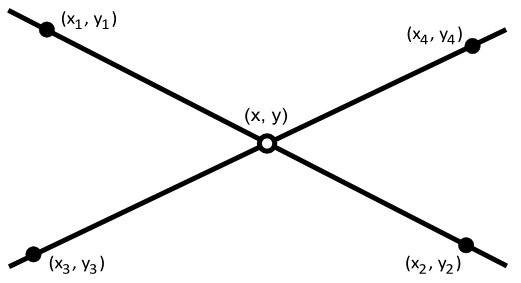
\includegraphics[height=2in]{Line-Line_Intersection.png}
%        \caption{Line line intersection}
%        \label{fig:linelineintersect}
%    \end{figure}
%}


 

\frontmatter 
\maketitle
\tableofcontents 
\chapter{Preface}

This book is intended as a reference, to be used both during the competition as well
in preparation for it.

It is hosted on github at
\href{https://github.com/VTACMProgrammingTeam/ICPCHandbook}{https://github.com/VTACMProgrammingTeam/ICPCHandbook}.
If you wish to contribute, please send email to godmar@gmail.com

The following authors have contributed to this book in its current form:
\begin{itemize}
    \item Godmar Back \texttt{<godmar@gmail.com>}
\end{itemize}
 

\mainmatter 
\chapter{Standard Libraries}

The ACM ICPC, at the time of this writing, allows the use of the JDK 1.6 libraries as well
as the C++ STL.  Knowledge and mastery of the existing JDK classes is crucial for success.
This chapter reviews some of the more commonly used classes.

\section{Collection Classes}

\subsection{Object Equivalence}
\label{sec:objequivalence}

Java allows you to define and equivalence relationship between objects using the
\code{Object.equals} method, which is required for some problems.  If implemented,
a conforming \code{hashCode} method must be implemented as well.
Here are some hints.

\begin{itemize}
\sloppypar
\item \textbf{Avoid gratuitous implementations.}  In the vast majority of cases,
you will not need your own \code{equals/hashCode} function!  You only need equals/hashCode
if your object is used as a key (not value!) in a Map or Set, \textbf{and} if the
default implementation of equals (``two objects are equal if they are the same'') does
not suffice.   Simply needing to store objects in a set, or using them as a map key,
is not a justification for implementing equals().
An example of where equals is needed are search problems in a state space - you may 
create a state instance that is equal to an already explored state kept track of
in a 'visited' set or map.

\item \textbf{Implement equals() correctly}.
You need to compare all relevant fields to one another.
\begin{minted}[fontsize=\footnotesize]{java}
@Override
public boolean equals(Object _that) {
    State that = (State)_that;
    return this.field1 == that.field1 && ... && this.fieldn == that.fieldn;
}

// or, as appropriate
@Override
public boolean equals(Object _that) {
    State that = (State)_that;
    return this.field1.equals(that.field1) && ... && this.fieldn.equals(that.fieldn);
}
\end{minted}
For clarity, I recommend for \code{equals()} to always consider all fields, and 
to not include irrelevant fields in the object.  (That is also why I like separate
previous hop maps rather than previous hop fields, or distance fields in BFS implementations,
see Section~\ref{sec:bfs}.)  The problem with selectively including some fields
in the comparison, and not others, is that it opens the door to mistakes in which
you accidentally use information from the wrong object.

\item \textbf{Understand the equals/hashCode contract}.
The contract says two objects that are equal must have the same hashCode().
It does not require that if two objects have the same hashCode() they must
be equals().  

\item \textbf{Implement hashCode() efficiently.} 
Rely on built-in functions, such as Arrays.hashCode() for arrays, or the built-in
hashCode() functions for Strings and Lists, which are known to be good.

\item \textbf{Consider hashCode()'s distribution.} 
The contract would be met by a degenerate function that returns always zero, but this
would create terrible performance - in a hash map, all objects would be mapped
to the same slot, resulting in linear lookup performance.
The chosen hash function should provide a distribution of hash values
that is as uniformly random as possible. 
Remember that Integer.hashCode does not use a 
\href{http://en.wikipedia.org/wiki/Fowler%E2%80%93Noll%E2%80%93Vo_hash_function}{Fowler-Noll-Vo}
hash, but rather returns the integer itself; the resulting randomness will be
small, especially if the number of items added dwarfs the range in which that integer varies.

When combining the hashes of fields, prefer bitwise xor (\^) over addition
or multiplication.  As an aside, it is not necessary that the lower bits are uniformly distributed -
Java's HashMap implementation does not perform a simple modulo, but rather draws
from higher-order bits, too:

\inputjava{javautilHashMap}

In my 2011/H Solution~\ref{sec:2011-h-rally}, execution time reduced from 87 to 29 
seconds by changing the hash function to use xor of all three components instead 
of multiplication of two components.

\end{itemize}

\subsection{Comparators}
\label{sec:comparators}

The most common uses of comparators are for sorting (Arrays.sort, Collections.sort, Collections.max, etc.), 
binary trees (java.util.TreeMap), and sorted queues (java.util.PriorityQueue).
Each use entails pitfalls.

\begin{itemize}
\item \textbf{Don't confuse partial orders with equality.}
    The contract of
    \href{http://docs.oracle.com/javase/6/docs/api/java/lang/Comparable.html#compareTo(T)}{compareTo}
    requires that the relationship be transitive across $<$, $>$, and $=$.  That implies, for instance, 
    that if $a > b \land b = c$ then $a > c$.
    When dealing with partial orders do not treat incomparable elements as equal.  Notably,
    in a partial order, it's well possible that $a < c$ if $a > b \land \lnot (b < c \lor b > c)$
    Instead, either complete the order or use topological sorting.

\item \textbf{Make the ordering consistent with equals.}
    A comparator should return 0 iff .equals() returns true.   This is required, in particular, when
    using TreeSets.  See \href{http://docs.oracle.com/javase/6/docs/api/java/lang/Comparable.html#compareTo(T)}{compareTo}.

\end{itemize}


\section{Arbitrary Precision Integers}

Java's \code{java.math.BigInteger} class provides support for arbitrary precision integer arithmetic.
(\href{http://docs.oracle.com/javase/6/docs/api/java/math/BigInteger.html}{JDK Doc}).
In addition to arbitrary precision integer arithmetic, this class provides

\begin{itemize}
    \item \textbf{Immutability.}  All operations return new BigIntegers.

    \item \textbf{Modular arithmetic.}  
        This includes computation of residues (\code{mod}), modular exponentiation (\code{modPow}),
        and even multiplicative inverse (\code{modInverse}).

    \item \textbf{Bit operations.}  BigInteger can be used as arbitrary-length bit vectors (and often make more sense
        than using java.util.BitSet, which is a mutable implementation!)
        Notable methods (in addition to \code{flipBit}, \code{clearBit}, \code{setBit}, \code{testBit}:
    \begin{itemize}
    \item \code{bitCount()} returns number of 1-bits for a positive number.
\begin{minted}[fontsize=\footnotesize]{java}
% System.out.println(BigInteger.valueOf(30).bitCount());
4
\end{minted}
    \item \code{bitLength()} returns position of highest set bit.
\begin{minted}[fontsize=\footnotesize]{java}
% System.out.println(BigInteger.valueOf(16).bitLength());
5
% System.out.println(BigInteger.valueOf(15).bitLength());
4
\end{minted}
    \item \code{getLowestSetBit()} returns position of lowest set bit.
\begin{minted}[fontsize=\footnotesize]{java}
% System.out.println(BigInteger.valueOf(30).getLowestSetBit());
1
% System.out.println(BigInteger.valueOf(31).getLowestSetBit());
0
\end{minted}
    \end{itemize}
        \item Support for \textbf{probabilistic primality testing}
            (using \href{http://en.wikipedia.org/wiki/Miller–Rabin_primality_test}{Miller-Rabin})
        via \code{isProbablePrime}, \code{nextProbablePrime}; support for GCD (via \code{gcd}).
    \item Like all \code{java.lang.Integer} and \code{java.lang.Long} it provides support for
        \textbf{base conversion} from/to strings for radices from 2 to 36.
\end{itemize}

\section{Bit Manipulation}

\textbf{\code{java.util.BitSet}} provides support for \textbf{mutable bit vectors} of arbitrary size.
Includes support for efficient iteration over set bits (\code{nextSetBit}); ditto for clear bits.
\begin{minted}[fontsize=\footnotesize]{java}
for (int i = bs.nextSetBit(0); i >= 0; i = bs.nextSetBit(i+1)) {
    // operate on index i here
}
\end{minted}

\textbf{\code{java.lang.Long.}}
An often overlooked class is \code{java.lang.Long}, which also provides support for
bit-twiddling on 64-bit longs.  Notable methods include
\begin{itemize}
\item \code{bitCount()} counts number of 1 bits.
\item \code{highestOneBit()} returns a long with only the highest bit set. (Note: unlike \code{BigInteger.bitLength()},
    this one returns not the position, but a long in which all other bits are cleared).
\begin{minted}[fontsize=\footnotesize]{java}
% System.out.println(Long.highestOneBit(16));
16
% System.out.println(Long.highestOneBit(15));
8
\end{minted}

\item \code{lowestOneBit()} returns long with only the lowest bit set.
\item \code{numberOfLeadingZeros} and \code{numberOfTrailingZeros} based on two's complement binary representation.
\begin{minted}[fontsize=\footnotesize]{java}
% System.out.println(Long.numberOfLeadingZeros(1));
63
% System.out.println(Long.numberOfLeadingZeros(1<<63));
0
% System.out.println(Long.numberOfLeadingZeros(2));
62
% System.out.println(Long.numberOfTrailingZeros(2));
1
\end{minted}

\item \code{reverse} reverse bits.
\end{itemize}

%%%%%%%%%%%%%%%%%%%%%%%%%%%%%%%%%%%%%%%%%%%%%%%%%%%%%%%%%%%%%%%%%%%%%%%%%%%%%%%%%%%%%%%
%
\section{Input}

The work horse for practically all input in ICPC problems is \code{java.util.Scanner}.  
Some notes on its recommended use.

\begin{itemize}
\item The default delimiter is always almost sufficient.  However, it can be changed.
    For instance, 2007/B Mobile's~\ref{sec:2007-b-mobile} input is free-formed S-Expressions
    spanning multiple lines, which are parsed using a delimiter that includes whitespace and
    a zero-width lookaround splitter, see Section~\ref{sec:lookaroundsplitting}.

\item Scanner does not support peeking at the next token without consuming it.
    Fortunately, this also isn't necessary in the vast majority of ICPC problems.  
    Should it be necessary, use the Scanner to fill an ArrayDeque of input tokens which
    can be peeked at.

\item Line-oriented vs. not Line-oriented input.  Many ICPC problems, though not all, use
    line-oriented input in which different pieces of information appear on different lines.
    Beware when mixing \code{nextLine()} and the other \code{next()} methods, such as \code{nextInt()}.
    For instance, to read the 2-line input
    \begin{verbatim}
    6 4
    orange
    \end{verbatim}
    into 2 ints and 1 string, the following calls would be necessary:
\begin{minted}[fontsize=\footnotesize]{java}
    int a = s.nextInt();    // read 6
    int b = s.nextInt();    // read 4, cursor is still one line 1
    s.nextLine();           // skip remainder of line
    String c = s.next();    // read orange; cursor now still on line 2
\end{minted}
    A recommended trick here is to nest Scanners and use only line-oriented 
    input on the outer scanner, like so:
\begin{minted}[fontsize=\footnotesize]{java}
    Scanner is = new Scanner(s.nextLine()); // read line with "6 4" and move to next line
    int a = is.nextInt();    // read 6
    int b = is.nextInt();    // read 4
    String c = s.nextLine(); // read orange and move to next line
\end{minted}
    This is particularly useful if parts of a line are optional, or depend on starting keywords.

\end{itemize}
 
\chapter{Simulation}

While many simulation problems can be solved ad-hoc, some require, or may benefit
from, a more principled approach.

\section{Monte Carlo Methods}

In some cases, random sampling might provide a solution.
For instance, the code below computes $\pi$ by examining whether
randomly produced $(x, y)$ samples are inside or outside the unit 
circle in the northeast quadrant.

\inputminted[fontsize=\footnotesize,linenos=true]{java}{code/Pi.java}

\paragraph{Precision} is generally not very good, mainly due to the  
statistical properties of the underlying pseudo-random number generator (PRNG).
Increasing the number of samples will yield diminishing returns quickly.
As a rule of thumb, don't expect more than 4 significant digits.
For example, 2010/Cells~\ref{sec:2010-c-cells} asks for a percentage with 2 digits after the
period, for a total of 4 significant digits, making this approach feasible.

\section{Discrete Event Simulation}

Discrete Event Simulation is widely used to simulate physical phenomena, especially
those that involve periodic and/or random events, as well as when the occurrence of
future events depends on the state of the simulated world, rather than being fixed
beforehand.

The key idea is to maintain a timeline as a queue of future events, sorted
by their timestamp.  Simulation time, aka virtual time, advances in jumps when
the next upcoming event is pulled off the queue.  Time jumps over period in which
no events are scheduled (unlike a continuous simulation in which time increases
in small, but constant, steps).

Event handlers may query the current time and they may schedule future events.
Discrete Event simulations contain a typical core: a way to represent events, 
a queue to sort them, and an event loop that processes the event queue until
either the maximum simulation time is reached or a solution to the problem is found.
Recommended implementation strategy is to use immutable event objects that are
inserted when scheduled and discarded after dispatch.

Example: \href{http://uva.onlinejudge.org/index.php?option=com_onlinejudge&Itemid=8&category=3&page=show_problem&problem=97}{UVA 00161}
is an example of a problem which can be solved with DES.  Note, however, that the small simulation time
frame (18,000 seconds) also allows a continuous simulation approach, simply simulating every second,
rather than only those points in time when a traffic light changes.
This is a very simple example, with only 3 event types, all implemented in one
class LightChange.

\inputminted[fontsize=\footnotesize,linenos=true]{java}{code/UVA00161TrafficLights.java}

 
\chapter{Searching}
\def\astar{$A^*$}

\section{Backtracking}
\label{sec:backtracking}
\index{Backtracking}

Bitner~\cite{Bitner:1975} first wrote up the underlying idea of backtracking in 1975.
While some ideas of that paper (notably, the use of macros) reflect specific implementation
ideas of that time, the rest is still relevant.

A canonical example of simple backtracking is to solve the N-Queens problem - arrange N queens
on a chessboard of size NxN such that no two can attack each other.  In this case, each
row must contain exactly one queen; the backtracking algorithm places queens on each square
in rows 1, 2, ..., N until the next queen either cannot be placed or a solution is found.

\inputjava{NQueens}

\paragraph{General Structure.}
The general structure of a backtracking function is
\begin{verbatim}
backtrack(<arguments that reflect partial solution> args)
{
    if (args say solution is found) {
        // process solution
        return <a solution was found>;
    }

    S = sort possible next steps by likelihood of finding a solution

    for (Steps s in S) {
        augment partial solution with s
        if (augmented solution is still feasible)
            backtrack(args');
        remove s from partial solution (undo)
    }
    return <no solution found>
}
\end{verbatim}
Alternatively, it is often convenient to clone the partial solution before augmenting it
with 's', which makes the undo step unnecessary.

\paragraph{Notes}
\begin{itemize}
\item Continue here.
\end{itemize}
 

\section{State Space Exploration}

In these problems, an initial state is to be transformed through a series of valid
moves into one goal state, or possibly one of multiple possible goal states. 
Examples include block puzzles or single-player games.
These problems have the following characteristics:
\begin{itemize}
\item An optimal solution required: we want the minimal number of moves from the
initial state to goal state, rather than just any.

\item No obvious strategy.  Given a state, there's no obvious way to choose which
move to make to get closer to the goal.  In fact, it's usually even difficult to
tell how far we might be away from the goal state.  Any easy-to-find lower bounds
for this distance to the goal might be far too optimistic.  
See also \astar{} in Section~\ref{sec:astar}.

\end{itemize}

\subsection{Breadth-First Search (BFS)}
\label{sec:bfs}
There are numerous ways of writing a BFS loop.  There are even more ways of
getting it wrong.
Here is one possible way:

\inputminted[fontsize=\footnotesize,linenos=true]{java}{code/bfsloop.java}

\paragraph{Notes.}  
\begin{itemize}
\item Adding the final state could be avoided by calling output() if a 
final state is found, potentially saving the unnecessary expansion of states
if the optimal goal state is already in the queue - however, then the case where 
the initial state is final must be handled separately.  
Seen in 2006/E Marbles~\ref{sec:2006-e-marbles} where the judge data contains
the case that the initial state is final.

\item The state class should use ducktyping and provide the necessary
methods - isfinal, successors.  In addition, the state class must implement
an object equivalence relationship (equals, hashCode) as described in 
Section~\ref{sec:objequivalence}.

\item The example keeps track of both the path (via 'pred') and distance (via 'dist').
    If the problem asks for only one of the two, the other can be omitted. In that
    case, the insertion of a successor state should be guarded by the one remaining.
    Note that both 'pred' and 'dist' have the invariant when encountering a state 
    multiple times, only the first encountered state is kept in the map.

\end{itemize}

\paragraph{When Not To Use BFS.}

There are some problems that may appear to be solvable using BFS, but are in fact 
dynamic programming problems.  These are generally problems in which there are
many transitions from states farther in the problem space to states that have
been discovered much earlier.
An example is 2007/C/Out of Sight.~\ref{sec:2007-c-sight}.

\subsection{\astar}
\label{sec:astar}

\astar~\cite{Pearl:1984} is a classic algorithm to improve upon breadth-first search when an
estimator function for states that estimates their distance to the goal state is known.
Though an AI algorithm, it can yield guaranteed optimal solution if the estimator is chosen
carefully.

The idea is simple.  In BFS, we're examining nodes based on their distance from the start state. 
So we'll look at, and expand, all states that are 6 moves away from the start *before* we 
look at any state that's 7 moves from the start - simply because of the FIFO discipline in the queue.

In \astar, instead of putting all to-be-explored states in a FIFO queue,
we sort them by their "goodness," which is defined as a
lower bound of how many moves a solution is away from the state.
For instance, if a state A is 6 moves away from the start, and
it is known that it is at least 10 moves away from the goal,
it would have a goodness of 16 (6 + 10).  On the other hand, if a
move B is 8 moves away from the start, and at least 4 moves away
from the solution, its goodness is 12 and it's explored first.
Note that we are not estimating how far the state is from
the solution. We're simply constructing a function that says: this
state is *at least* this far from a solution. It may be farther -
our decision to explore state B may be wrong and the closest solution
state may result from the exploration of A.

The challenge lies in how to say - quickly - that a state is
``at least this many moves away from the goal.''  In general, that's
tough since if we knew how many states a state is away from the goal,
it would be much easier to solve the problem. However, there are some lower
bounds that can be found - for instance, in a puzzle, we could count how
many pieces are not in their final position, knowing that it'll take at
least this many moves to get them there (assuming it's a puzzle like
the traditional 15-piece puzzle where all pieces need to be sorted).
Another possible function is the sum of the Manhattan
distances between each piece's current and final position.  
Again, it is clear that it will take at least this many moves.

In competition problems you are practically never asked to find an 'almost'
perfect heuristic solution - they ask
you to compute the correct, and in search problems like these, the
shortest solution.  \astar{} will provide you with the optimal
solution if the estimation function does not overestimate  - if it
did, it might lead to the nearest goal state being placed behind a
farther goal state in the queue.  That farther state might then be
discovered first, and mistaken for the shortest solution.

It's not a problem that the estimation function underestimates - in fact,
it'll generally do that - this just means that \astar might waste some
time exploring states it thinks are promising, but which do not actually
lead to a solution.

Converting a BFS to A-Star in Java is really simple.  Replace the entry
of the BFS described in Section~\ref{sec:bfs} such that the BFS work
queue uses a PriorityQueue like so:

\inputminted[fontsize=\footnotesize,linenos=true]{java}{code/astar.java}

Note how making dist final allows it to be used in the comparator.
The code exploits that both PriorityQueue and ArrayDeque implement the
Queue interface.

\paragraph{Notes}  
\begin{itemize}
\item
\astar will increase the cost of inserting and removing a state from the queue
substantially - in a heap-based priority queue, 'offer()' and 'poll()' take O(log n) whereas 
they are constant time O(1) operations on a Deque.  On the other hand, especially if the
estimator function is too optimistic, the state space may only be marginally reduced.
Recommendation: use A-Star only if BFS times out and/or if a good heuristic
can be found.

\end{itemize}
 
\chapter{String Processing}

\section{Regular Expressions}

\subsection{Regular Expressions}

\subsection{Zero-width Lookahead Technique}
\label{sec:lookaroundsplitting}

\begin{figure}
    \centering
    % Wikipedia Public Domain image
    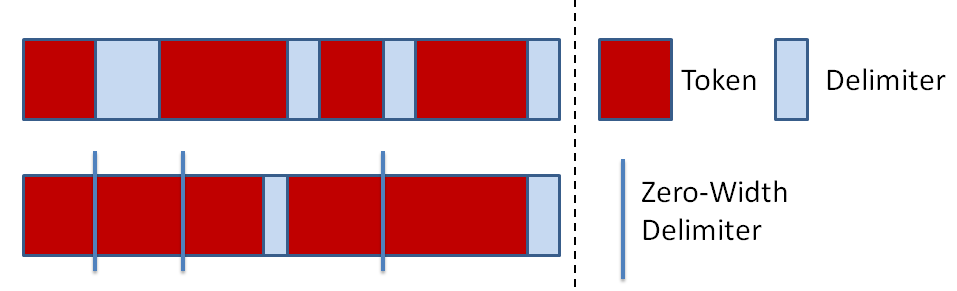
\includegraphics[height=1.5in]{lookaheadsplitting.png}
    \caption{Lookahead Splitting. The top shows a traditional scanner/split which consumes delimiters.
    The bottom shows a scanner using delimiter expressions that may or may not consume characters.}
    \label{fig:lookaheadsplit}
\end{figure}

In some problems (notably, 
      2007/B/Mobile~\ref{sec:2007-b-mobile}, 
      2007/D/Witness~\ref{sec:2007-d-witness}, 
      and 2008/G/Stems~\ref{sec:2008-g-stems}),
the string and/or input handling of these problems can greatly 
benefit from using zero-width positive lookahead/lookbehind regular expressions.

To understand how they work, consider how java.util.Scanner works. By
default, a Scanner splits the input stream into tokens using a delimiter
pattern. The default delimiter pattern is one or more whitespaces
(written as \verb!\p{javaWhitespace}! or, when embedded in Java code, as
\verb!"\\p{javaWhitespace}+"!). The input characters that are matched by the
delimiter itself are consumed by the Scanner – there is no way to
retrieve them.

In some cases, whitespace is not a suitable delimiter. Suppose
you're asked to parse an arithmetic expression that uses +, -, *,
and /. Whitespaces are optional, so both \verb!1+1! and \verb!1 + 1! as well as 
\verb!1 +1! are valid expressions. If you made the operators '+', '-'
etc. delimiters (perhaps in addition to whitespace), a Scanner would
retrieve '1' and '1', but there would be no way to retrieve the
'+' – so you couldn’t distinguish '1+1' and '1-1'.  Instead, use
lookaround matching by adding a zero-width delimiter that matches before
or after a +, -, *, or /.  ``Zero-width'' here means that although
the delimiter matches (and thus causes the Scanner to stop and return
what it has read so far!), it does not consume any characters. Thus,
the scanner will stop, but the delimiter (which the Scanner swallows)
has zero width – therefore, the characters are returned as part of
the previous token. In this example, s.next() would return '+'.

Figure~\ref{fig:lookaheadsplit} shows a traditional scanner (top) and a scanner that
uses both consuming and non-consuming delimiters (bottom): Note that
if the delimiter used by the scanner does not consume any characters,
the scanner will return the entire input stream. This is very useful if
you need to manipulate a stream without losing any characters.

The idea to use String.format to turn any regular expression into a 
zero-width lookahead or lookbehind delimiter is taken from \href{http://stackoverflow.com/questions/2206378/how-to-split-a-string-but-also-keep-the-delimiters}{here}.

Note that this technique can be used with a java.util.Scanner object
(via useDelimiter), but also in all other functions that use regular
expressions as delimiters, notably String.split().

Finally, note that you cannot use some regular expressions to describe
zero-width delimiters. Notably, \textbf{expressions using repetition (* or +)
cannot be used.}

\paragraph{Code Example.}
The following program shows some of the applications of
this style of matching.  These examples include:
\begin{itemize}
\item Arithmetic expressions with optional whitespace
\item S-Expressions with optional whitespace before and after ( )
\item Finding words in a sentence
\item Finding sentences in a paragraph
\end{itemize}

\inputminted{java}{code/Lookaround.java}

\subsection{NFA Simulation}
\index{NFA!Simulation}

The Regex engine in Java does not convert to a Thompson-DFA; it uses a backtracking algorithm
to find out if a regular expression matches a string.  This leads to pathological cases with
exponential runtime increase, particularly when the regular expression contains a large number
of Kleene stars.

In those situations, it may be helpful to construct your own mini-regexp interpreter by building
and simulating an NFA (nondeterministic finite automaton).

Example problem is \href{http://ncpc.idi.ntnu.no/ncpc2011/ncpc2011problems.pdf}{NCPC 2011/E}
where the input are globs such as \texttt{*a*a*a*a} that should be matched against filenames.
Figure~\ref{fig:nfaexample} shows an example of how to construct such a NFA.
In an NFA there may be multiple transitions labeled with the same symbol: for instance,
there's a transition labeled 'b' from state 0 to state 1, but there is also a transition
labeled 'b' from state 0 to state 0.  For the input string \texttt{abc}, the 'b' would
transition into state 1, whereas for the input string \texttt{abbc}, the first 'b' would
transition into state 0, the second into state 1.

Of course, we don't know which it's actually going to be - a NFA, in its theoretical 
formulation, is defined to oracle-like pick the correct transition.  That's why we simulate
it by simply keeping track of all possible (``active'') states the NFA might be in after each symbol.
This is done using a set (HashSet or BitSet if the states are nicely numbered).
For each input symbol, we compute the possible set of successor states based on the
current set of active states.  If after the string has been exhausted the goal state
is in the set of active states the string is matched.
A Python solution is shown below for succinctness.

\begin{figure}
    \centering
    % Wikipedia Public Domain image
    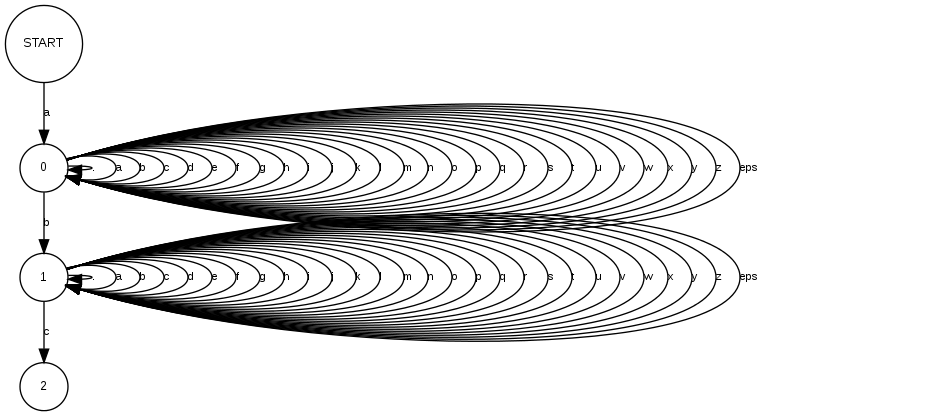
\includegraphics[height=3in]{a-star-b-star-c.png}
    \caption{NFA for regular expression \texttt{a.*b.*c} representing glob \texttt{a*b*c}
        over alphabet of lowercase letters and period (.)}
    \label{fig:nfaexample}
\end{figure}

\inputminted{python}{code/ls.py}

\section{Parsing}
\subsection{Recursive Descent}

 
\chapter{Mathematics}

\section{Combinatorics}

A number of problems require basic knowledge of combinatorics.  
We have seen two characteristics of these problems:
\begin{itemize}
\item They are designed such that brute-force approaches that include the enumeration of
    permutations or combinations will time out.  A telltale sign is if the problem allows
    ranges for its input parameters that exceed 32 bits ($2^{32} \sim 4 x 10^9$) or allow
    for up to $10^{18}$.  Reminder: $2^{63} \sim 9 x 10^{18}$
\item Because the input sizes are such that brute-force enumeration is ruled out, there
    is a risk of integer overflow when computing binomial cofficient and factorials.
\end{itemize}

\index{Permutations}
\textbf{Permutations of length $k$ of $n$ elements, allowing for repetitions}: 
\[
    n^k
\]
Important special case is $n=2$ - number of permutations
of length $k$ is equal to number of ways in which to form $k$ bits ($2^k$).

\textbf{Permutations of $n$ elements, no repetitions}: 
\[
    n! = n (n-1) (n-2) \ldots 1
\]

\inputjava{bigintegerfactorial}

\index{Factorial}
\textbf{Number of unique permutations when elements occur multiple times.}  Assume $a_i$ may be repeated $k_i$ times. 
    Let $L = \sum_{i = 1}^{n} k_i$ the sum of their frequencies.

\[
    \frac{L!}{k_1! k_2! \ldots ... k_n!}
\]
Example: unique permutations of (aabb) is $L = 4$, so $\frac{4!}{2! 2!} = 6$.  The permutations are
(aabb), (abab), (abba), (baab), (baba), (bbaa).

\index{Combinations}
\index{Binomial Coefficient}
\textbf{Combinations of $k$ out of $n$ elements, no repetition}:
\[
    \binom{n}{k} = \frac{n!}{k! (n-k)!}
\]

Aside: C++ is a valid language at the ICPC, but unlike Java, C++ does not have a standard
library for arbitrary-size integers that is accessible during the contest.  This has led to problems in which
the problem states that the result fits into a 64-bit long, but where the straightforward
application of the formula for $n!$ or $\binom{n}{k}$ would lead to integer overflow.

In those cases, it is recommended to perform the arithmetic in BigInteger and then convert
down if/when needed, as in the example below:

\inputjava{bigintegerbinom}

Note that Java does not have an unsigned 64-bit type, so above code will fail for 
coefficients that are $2^{63} \leq \binom{n}{k} < 2^{64}$.  
For the same reason, however, judge data usually avoids that range.
Code above is from solution to 2010/D Bit~\ref{sec:2010-d-bit}

\textbf{Combinations of $k$ out of $n$ elements, can repeat any element any number of times}:
\[
    \binom{n + k - 1}{k}
\]

 
\chapter{Geometry}

\section{Basics}

A determinant of a $2x2$ matrix is defined as
\[
    \left\vert
        \begin{array}{cc}
            a & b \\
            c & d \\
        \end{array}
    \right\vert
    = a d - b c
\]

\section{java.awt.geom}

The \texttt{java.awt.geom} and \texttt{java.awt} packages have, albeit limited, facilities
for geometric problems.  There are classes to represent shapes - see
\href{http://docs.oracle.com/javase/6/docs/api/java/awt/Shape.html}{java.awt.Shape}, including
lines, ellipses, rectangles and some curves.

\begin{itemize}
\item "is contained in".  java.awt.geom.Shape provide a contains() method to test if a point
    is contained in a shape.  Contains() returns true if the point is in the interior, and false
    if the point is outside the shape. However, it \textbf{may return true or false if the point is 
    on the shape boundary.} 

\begin{figure}
    \centering
    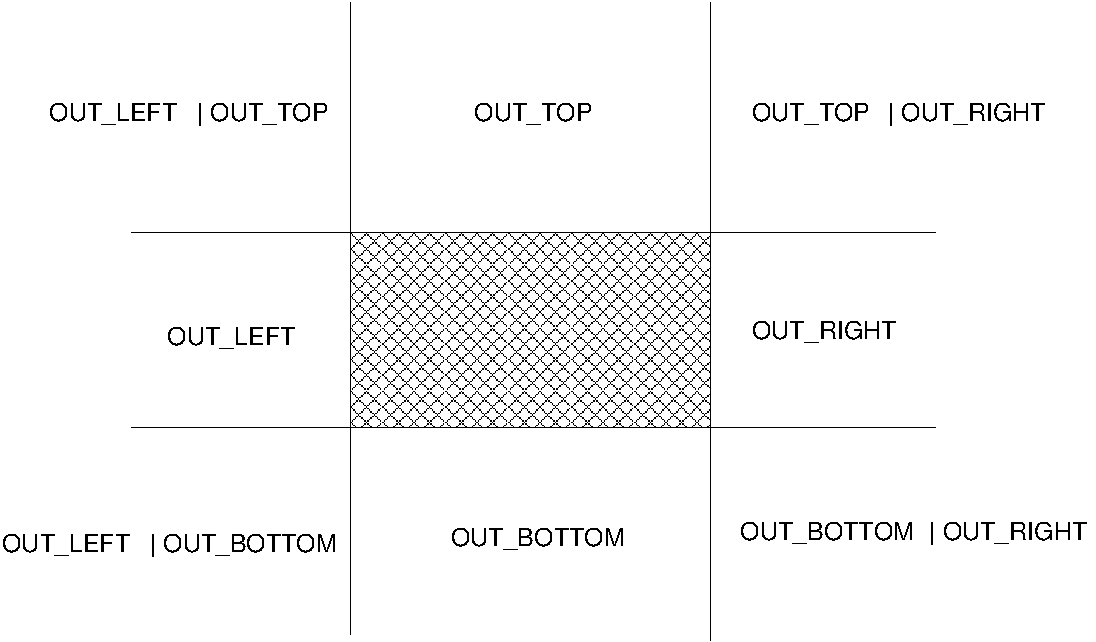
\includegraphics[height=2in]{outcode.pdf}
    \caption{Outcode - note that points that lie on any of the sidelines are considered inside.}
    \label{fig:outcode}
\end{figure}

\item "outcode". Outcodes were invented by Cohen-Sutherland; they are used for clipping
    in computer graphics.  java.awt.geom.Rectangle2D provides an outcode() method.
    The result is 0 if a point is inside or on any sideline of the rectangle; otherwise 
    the result is a
    combination of bits that represent where the point lies in relationship to the
    rectangle, as shown in Figure~\ref{fig:outcode}.
    For clipping of lines, the outcodes of the start and end point are
    computed, which then allows a quick identification of whether the line is inside,
    must be clipped, may be ignored, or needs further investigation.
    A useful property of outcode() is that it can substitute as a replacement for
    contains() in case where a point may lie on an edge but should be considered
    inside. 

\item "intersects."  Tests if a shape intersects with a rectangle.
    Can also test if two lines or line segments intersect, but cannot find the point of
    intersection.

\item "is point on line segment." Implements this as Line2D.ptSegDistSq(Point2D) $<$ 1e-9.

\end{itemize}

\section{Coordinate Geometry}

\subsection{Line/Line Intersection}
\label{sec:lineintersection}
\index{Line/Line Intersections}

\begin{figure}
    \centering
    % Wikipedia Public Domain image
    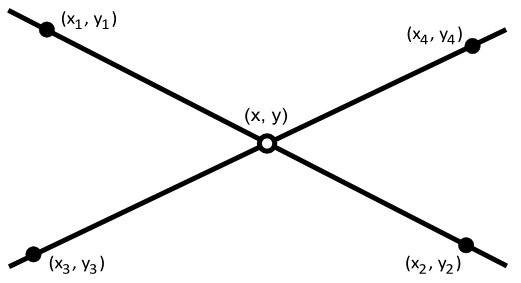
\includegraphics[height=1.5in]{Line-Line_Intersection.png}
    \caption{Line line intersection}
    \label{fig:linelineintersect}
\end{figure}

\[
\begin{array}{ll}
P_x = \frac{\begin{vmatrix} 
                \begin{vmatrix} x_1 & y_1\\
                                x_2 & y_2
                \end{vmatrix} & 
                \begin{vmatrix} x_1 & 1\\
                                x_2 & 1
                \end{vmatrix} \\\\ 
                \begin{vmatrix} x_3 & y_3\\
                                x_4 & y_4
                \end{vmatrix} & 
                \begin{vmatrix} x_3 & 1\\
                                x_4 & 1
                \end{vmatrix} 
            \end{vmatrix} }{
            \begin{vmatrix} 
                \begin{vmatrix} x_1 & 1\\
                               x_2 & 1
                \end{vmatrix} &  
                \begin{vmatrix} y_1 & 1\\
                                y_2 & 1
             \end{vmatrix} \\\\ 
             \begin{vmatrix} x_3 & 1\\
                             x_4 & 1
             \end{vmatrix} & 
             \begin{vmatrix} y_3 & 1\\
                             y_4 & 1 
             \end{vmatrix} 
            \end{vmatrix}}

&

P_y = \frac{\begin{vmatrix} 
                \begin{vmatrix} x_1 & y_1\\
                                x_2 & y_2
                \end{vmatrix} &  
                \begin{vmatrix} y_1 & 1
                              \\y_2 & 1
                \end{vmatrix} \\\\ 
                \begin{vmatrix} x_3 & y_3\\
                                x_4 & y_4
                \end{vmatrix} & 
                \begin{vmatrix} y_3 & 1\\
                                y_4 & 1
                \end{vmatrix} 
            \end{vmatrix} }
           {\begin{vmatrix} 
               \begin{vmatrix} x_1 & 1\\
                               x_2 & 1
               \end{vmatrix} &
               \begin{vmatrix} y_1 & 1\\
                               y_2 & 1
            \end{vmatrix} \\\\ 
            \begin{vmatrix} x_3 & 1\\
                            x_4 & 1
            \end{vmatrix} & 
            \begin{vmatrix} y_3 & 1\\
                            y_4 & 1
            \end{vmatrix} 
     \end{vmatrix}}\,\!
\\

\end{array}
\]

The determinants can be written out as:
\begin{align*}
    (P_x, P_y)= \bigg(&\frac{(x_1 y_2-y_1 x_2)(x_3-x_4)-(x_1-x_2)(x_3 y_4-y_3 x_4)}{(x_1-x_2)(y_3-y_4)-(y_1-y_2)(x_3-x_4)}, \\
                      &\frac{(x_1 y_2-y_1 x_2)(y_3-y_4)-(y_1-y_2)(x_3 y_4-y_3 x_4)}{(x_1-x_2)(y_3-y_4)-(y_1-y_2)(x_3-x_4)}\bigg)
\end{align*}

Source: \href{http://en.wikipedia.org/wiki/Line-line_intersection}{http://en.wikipedia.org/wiki/Line-line\_intersection}.

\paragraph{Notes}
\begin{itemize}
\item Does not handle parallel or coincident lines:
    Denominator will be zero:
    \[
        (x_1 - x_2) (y_3 - y_4) - (y_1 - y_2) (x_3 - x_4) = 0
    \]
\item Does not handle if lines are each others' normal (i.e., at a right angle).
    If line is horizontal ($y_1 = y_2$ or $y_3 = y_4$), and the other vertical ($x_1 = x_2$ or $x_3 = x_4$) 
    denominator will also be a 0 determinant, but the lines will intersect.  
    Handle as special case if problem allows it.

\item Intersection point may be outside the given segments.

\item If you only need to know if two lines intersect, but not where, use java.awt.geom.Line2D.intersects.
\end{itemize}

\paragraph{Code}

This code is from a solution to 2011/F (Section~\ref{sec:2011-f-lineofsight}) where the 
parallel and rectangular cases do not occur. (TBD: provide complete implementation.)

\inputminted[fontsize=\footnotesize,linenos=true]{java}{code/lineintersection.java}

%
%
%

\subsection{Area of a Polygon}
\label{sec:areapolygon}
\index{Polygon!Area}
\index{Area!Polygon}
\index{Polygon}

The signed area of a planar non-self-intersecting polygon with vertices $(x_1, y_1), \dots, (x_n, y_n)$ is
\[
    A = \frac{1}{2} \left(
        \left\vert
        \begin{array}{cc}
            x_1 & x_2 \\
            y_1 & y_2 \\
        \end{array}
        \right\vert
        +
        \left\vert
        \begin{array}{cc}
            x_2 & x_3 \\
            y_2 & y_3 \\
        \end{array}
        \right\vert
        + \ldots +
        \left\vert
        \begin{array}{cc}
            x_n & x_1 \\
            y_n & y_1 \\
        \end{array}
        \right\vert
        \right)
\]

Figure~\ref{fig:polygonareadeterminant} shows how to multiply this out
\[
    A = \frac{1}{2} \left(
        x_1 y_2 - x_2 y_1
      + x_2 y_3 - x_3 y_2
      + \ldots +
      + x_{n-1} y_n - x_n y_{n-1}
      + x_{n} y_1 - x_1 y_n
      \right)
\]

(Source: Mathworld~\cite{mathworldpolygonarea})

\begin{figure}
    \centering
    % Wikipedia Public Domain image
    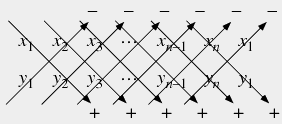
\includegraphics[height=1.5in]{PolygonArea_1000.png}
    \caption{Line line intersection}
    \label{fig:polygonareadeterminant}
\end{figure}

\paragraph{Notes}
\begin{itemize}
\item Works for any simple polygon (concave or convex)
\item Does not work for complex polygons (when any edges intersect)
\item Points \textbf{must be ordered} if polygon has more than 3 vertices, or output is junk.
\item A is positive if points are in counterclockwise order, negative if points are in clockwise order.
    See the use of Math.abs() in code below.
\item Triangle and any Quadrilateral are, of course, just special cases.
    For triangles, order does not matter.
\end{itemize}

\paragraph{Code}
\inputminted[fontsize=\footnotesize,linenos=true]{java}{code/polygonarea.java}

Special case of a triangle:

\inputminted[fontsize=\footnotesize,linenos=true]{java}{code/triangleareacoord.java}

 
\chapter{Gotchas}

Common mistakes and idiosyncrasies observed in the judge input and specification of
various problems posed at competitions.

\begin{enumerate}
\item \textbf{Judge input not terminated as required}. Typically, the problem states that
    there's some way to identify the end of input without having to rely on EOF.
    We've observed judge input, however, where EOF terminated the input.
    You should try to write your input loop such that your solution works whether
    the input is terminated by EOF or by the specified end-of-input delimiter.
    This strategy may allow you to submit a correct solution even before the mistake
    is discovered (and may even lead to a delay in when it's discovered that would benefit
    your team.)
    Seen in 2006/E Marbles~\ref{sec:2006-e-marbles}.

\item \textbf{Trailing Spaces}.
    In problems that state "there is one word per line" we have observed trailing spaces
    which must be trimmed.   Advice: always use String.trim(), unless the spaces are
    significant, which we have not seen anywhere.
    Seen in 2007/D Witness~\ref{sec:2007-d-witness}.

\item \textbf{Leading Spaces}.
    In some problems, (insignificant) leading spaces may occur.  The catch here is that 
    naive splitting without trimming may produce an empty string in the first position.
    See bsh output below:
    \begin{Verbatim}
    % System.out.println(Arrays.toString("  word1  word2  ".split("\\s+")));
    [, word1, word2]
    \end{Verbatim}
 
    Seen in 2011/B Raggedy~\ref{sec:2011-b-raggedy}.

\end{enumerate}

 
\chapter{Mid-Atlantic Problem Sets}

This chapter contains some notes about the problems occurring in the Mid-Atlantic
problem set.  We focus on this corpus in particular because there are recurring
themes since the problems have been created by the same person (or team) for
multiple years.

\section{2005}

\href{(Problem PDF 2005)}{http://midatl.radford.edu/docs/pastProblems/05contest/MidAtlantic2005.pdf}

\subsection{C Extrusion}
\label{sec:2005-c-extrusion}

Straightforward application of polygon area formula, see Section~\ref{sec:areapolygon}.

\section{2006}
\href{(Problem PDF 2006)}{http://midatl.radford.edu/docs/pastProblems/06contest/MidAtlantic2006.pdf}

\subsection{E Marbles}
\label{sec:2006-e-marbles}
A simple state space exploration problem solvable with straightforward BFS exploration.
Catch: judge input data missed the "0 0 0" line.

\section{2007}
\href{(Problem PDF 2007)}{http://midatl.radford.edu/docs/pastProblems/07contest/MidAtlantic2007.pdf}

\subsection{B Mobiles Alabama}
\label{sec:2007-b-mobile}

Lexical analysis benefits from zero-width lookaround~\ref{sec:lookaroundsplitting}, although
simpler solutions (replacing '(' and ')' with ' ( ' and ' ) ' before splitting on whitespace
may work, too.
Recursive descent parsing should be used to analyse the syntactical structure of the input.

\subsection{D Witness Redaction}
\label{sec:2007-d-witness}
This problem can be solved with regular expressions and zero-width lookaround splitting.
See Section~\ref{sec:lookaroundsplitting}.

\section{2008}
\href{(Problem PDF 2008)}{http://midatl.radford.edu/docs/pastProblems/08contest/MidAtlantic2008.pdf}

\subsection{G Stems Sell}
\label{sec:2008-g-stems}

Can be solved with regular expressions.

\href{Judge data}{http://midatl.radford.edu/docs/pastProblems/08contest/JudgingData/G-stems/}
appears broken, even on ICPC site.

\section{2011}

\href{(Problem PDF 2011)}{http://midatl.radford.edu/docs/pastProblems/11contest/MidAtlantic2011.pdf}

\subsection{B Raggedy, Raggedy}
\label{sec:2011-b-raggedy}

This problem can be solved using dynamic programming.
Note that there may be leading spaces on some input lines.

\subsection{F Line of Sight}
\label{sec:2011-f-lineofsight}

Straightforward application of area of polygon~\ref{sec:areapolygon} and line intersection~\ref{sec:lineintersection}.
Note that parameters of the problem even exclude corner cases for line intersection (e.g. parallel lines, right angles).

 

\backmatter 
%\include{glossary} 
%\include{notat} 

\bibliographystyle{plain} %The style you want to use for references. 
\bibliography{references} %The files containing all the articles and books you ever referenced. 

\printindex

\end{document}

